

\chapter{实验结果及分析}

\section{测试样例}

如图\ref{fig:pipelining},我们在request\_pipeline中客户端同一个TCP向服务器发送多个并发请求。我们根据服务器返回的实验结果来看(以最后几个为例)。第一个请求是GET方法,格式等也均是正确的,服务器也能正确解析返回给客户端消息;而第二个是HAHA方法,这个我们没有实现过,即返回“HTTP/1.1 501 Not Implemented\textbackslash r\textbackslash n\textbackslash r\textbackslash n”。

而第三个是/~prs/15-441-F15/HTTP/1.1,存在格式错误,因此服务器返回“HTTP/1.1 400 Bad request\textbackslash r\textbackslash n\textbackslash r\textbackslash n”。服务器能够识别这个错误请求并拒绝了这个请求,也能继续识别并发的下一条请求。下一条请求HTTP/1.30也存在格式错误,同样,服务器能够在拒绝上一条错误请求之后解析这条这条请求。根据结果来看,我们的实现是正确的。对于这个结果,我们也容易从代码分析出来这是正确的。我们引入了strstr(str,dest)函数,我们就能找到”\textbackslash r\textbackslash n\textbackslash r\textbackslash n”的位置。找到了”\textbackslash r\textbackslash n\textbackslash r\textbackslash n”的位置之后,也很容易找到单个报文,我们之前已经实现了正确解析单个报文。所以我们处理出来了单个报文之后也就能正确处理这些并发的请求了。

\begin{figure}[htbp!]
    \centering 
    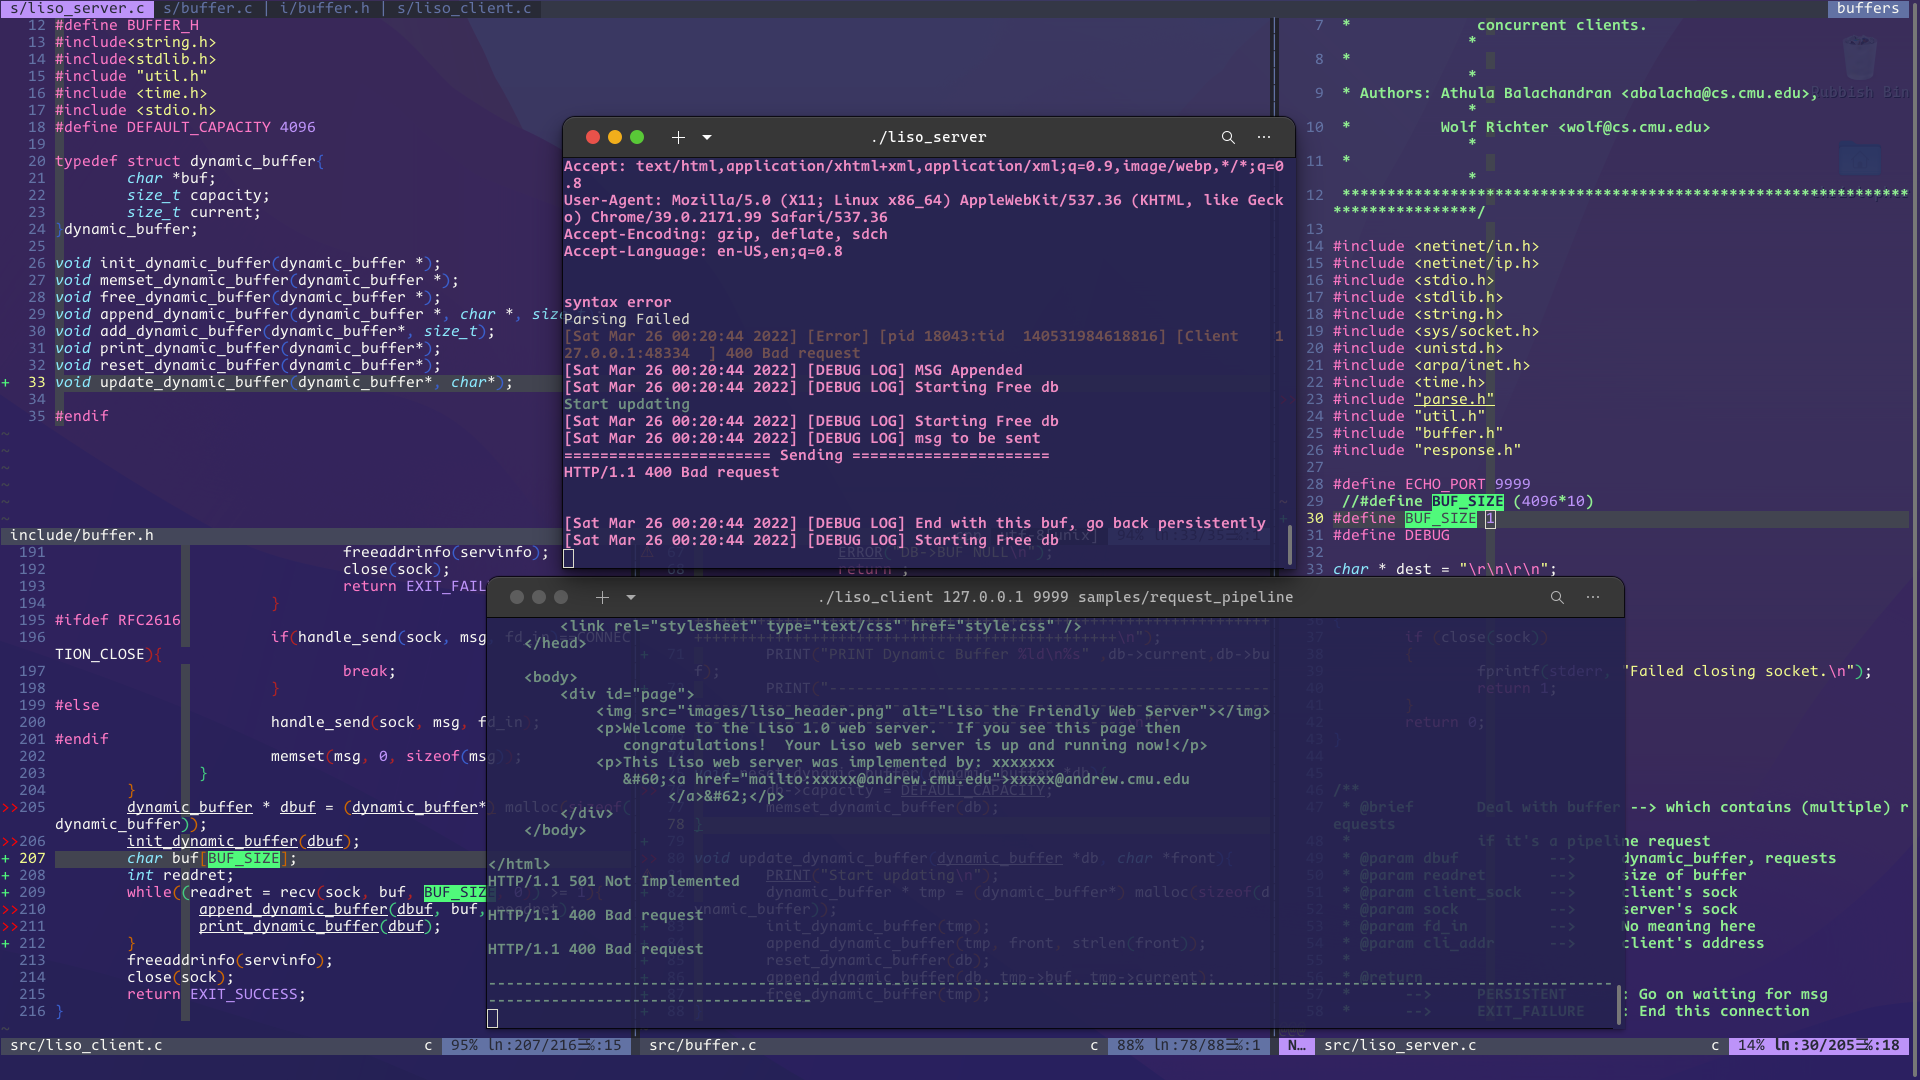
\includegraphics[width=5in]{BUF=1.png}
    \caption{pipelining test}
    \label{fig:pipelining}
\end{figure}

autolab的测试如图\ref{fig:autolab3} 所示。

\begin{figure}[htbp!]
    \centering
    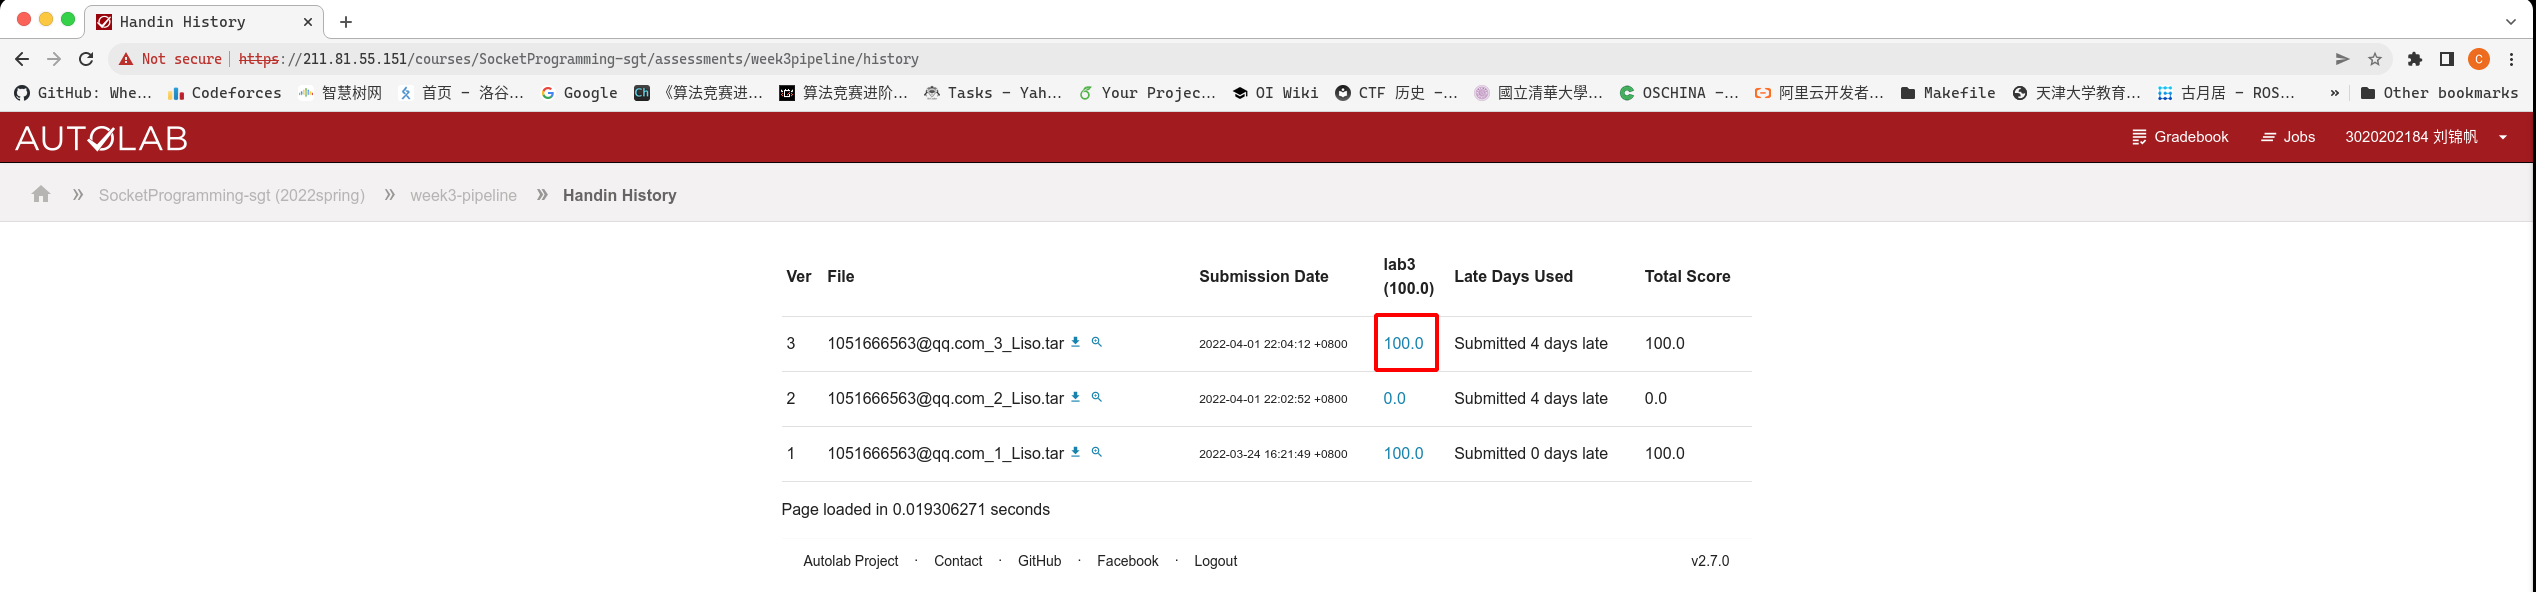
\includegraphics[width=5in]{autolab3.png}
    \caption{Autolab Test Result}\label{fig:autolab3}
\end{figure}